\section{动态放置机制的研究进展与比较}
\label{sec:research}

\subsection{基于专家拉取的数据中心化训练}

Janus\cite{ref1}首先重新选择了通信对象。固定专家方式移动大量 token 或 activation，Janus 则让数据保留在原 worker，根据当前路由按需拉取对应专家权重，并用缓存、机内共享、预取、拓扑优先级和异步任务重叠通信与计算。其成立的关键条件是，需要传输的 token 数据量大于可复用的专家权重，并且权重拉取不会因拷贝和调度产生新的暴露等待。

在 32 张 A100 上，Janus 报告最多 16 倍流量减少和 2.06 倍迭代加速\cite{ref1}。这些结果支持``改变通信对象能够改变网络代价''的判断，但 Janus 的机制是按需取得计算所需的权重，而非把热门 expert 永久迁移或复制到更多 GPU：反向阶段仍要把梯度送回原始 worker。因此，专家尺寸、batch 或 sequence 规模、权重复用和缓存命中情况决定了拉取是否有利；当权重不再小于需要交换的 token 时，原有以专家为中心的通信方式可能重新具有竞争力。

\subsection{面向负载均衡的动态专家放置}

FasterMoE、FlexMoE 和 SYMI 面向的是热门 expert 造成的计算、容量和排队压力。FasterMoE 用性能模型和 DDL-Roofline 判断何时对热门专家做 shadowing，并把 All-to-All 与专家计算拆成可重叠任务\cite{ref5}。FlexMoE 将扩展、收缩和迁移纳入放置决策，通过增加热门专家副本分摊 token；其 64 张 A100 实验相对 DeepSpeed 平均 1.70 倍、最高 2.10 倍，相对 FasterMoE 平均 1.30 倍、最高 1.45 倍\cite{ref2}。两类方法的收益来源都是增加热门专家的可用计算槽位，而不是直接让所有 token 留在本地。

副本扩张随之引入状态问题：权重需要分发，副本梯度需要同步，迁移还可能涉及优化器状态；若热点持续时间过短，重配置成本可能无法被后续收益摊销。

专家容量还关联 token dropping 和训练收敛。SYMI 的 16-GPU GPT-Small 设置中，容量系数为 ×1、×2、×4 时，token survival 分别为 44.90\%、65.56\%、74.91\%，达到目标 loss 分别需要 618、527、478 次迭代，前向延迟为 455.41、506.77、571.42 ms\cite{ref4}。这表明专家复制的评价不能只看单步时间，还要同时观察 token 接纳率和训练进展。

SYMI 把优化器状态静态分片，同时根据 popularity 调整 GPU 上的专家权重或实例放置，降低状态随专家移动的约束。该结果体现状态解耦与动态放置的结合，不意味着副本不再需要权重、梯度或集合通信；其设计复用了正常优化器更新中本来就要发送的更新权重。论文在 16 张 A100 GPU 的评测中报告，GPT-Small 达到 loss 4.0 时，DeepSpeed 为 147.84 分钟，SYMI 为 102.68 分钟；相对 DeepSpeed 和 FlexMoE 的 time-to-convergence 分别快 30.5\% 和 25.9\%，并报告相对系统少丢 43\%--69\% 的 token\cite{ref4}。这些结果不能归因于单一因素。

\subsection{基于路由局部性的动态样本放置}

NetMoE\cite{ref3}从样本一侧处理跨节点路径。它利用同一样本的 token 可能具有路由局部性，先决定样本的节点，再决定节点内设备，使部分 token 在目标节点内完成后续交换。NetMoE 不先执行独立的跨节点样本迁移，而是把新的设备分配融合到当前层 All-to-All Gather，使专家输出直接落到新的样本位置；由于该位置会成为下一层输入，优化目标同时包含当前层 Gather 与下一层 Scatter。

为保证重排不破坏 Transformer 的残差语义，NetMoE 使用 expert residual inlining，将残差加法安排在 Scatter 之后、Gather 之前。为满足在线训练的时间要求，它将放置求解转化为加权二分图匹配，用 Kuhn-Munkres 在 CPU 后台运行，并与 scatter 和专家计算重叠。因而主要代价是既有 Gather/下一层 Scatter 的目的地重定向、索引与残差映射维护及匹配求解，而不是额外的大规模搬运。

在 4 节点、32 张 A800-SXM4 40 GB 的实验中，NetMoE 在 50 次迭代平均设置下最高相对 FastMoE、FasterMoE 和 SmartMoE 加速 1.67、1.37 和 1.33 倍；在 Table 4 的 MoE-GPT-S、16 GPU、I/J=2 求解器对比中，KM 为 0.08 ms、PuLP 为 42.8 ms\cite{ref3}，不等同于上一句 32 GPU 实验的通用开销。样本位置可用于网络优化，但重排不消除 All-to-All：它仍需维护样本、序列、残差和微批对应关系，只在局部性和机内外带宽差异存在时减少跨节点部分。

\subsection{不同动态放置机制的综合比较}

三类放置对象的差别在于移动对象和释放资源：专家拉取改变数据与权重的交换对象，专家复制增加热门专家的计算位置，样本重排改善 token 与 expert 的拓扑映射；通信调度是可叠加的执行层，调整已有通信顺序。图~\ref{fig:mechanisms} 展示四项工作的决策链路与调整成本。

\begin{figure}[!htbp]
\centering
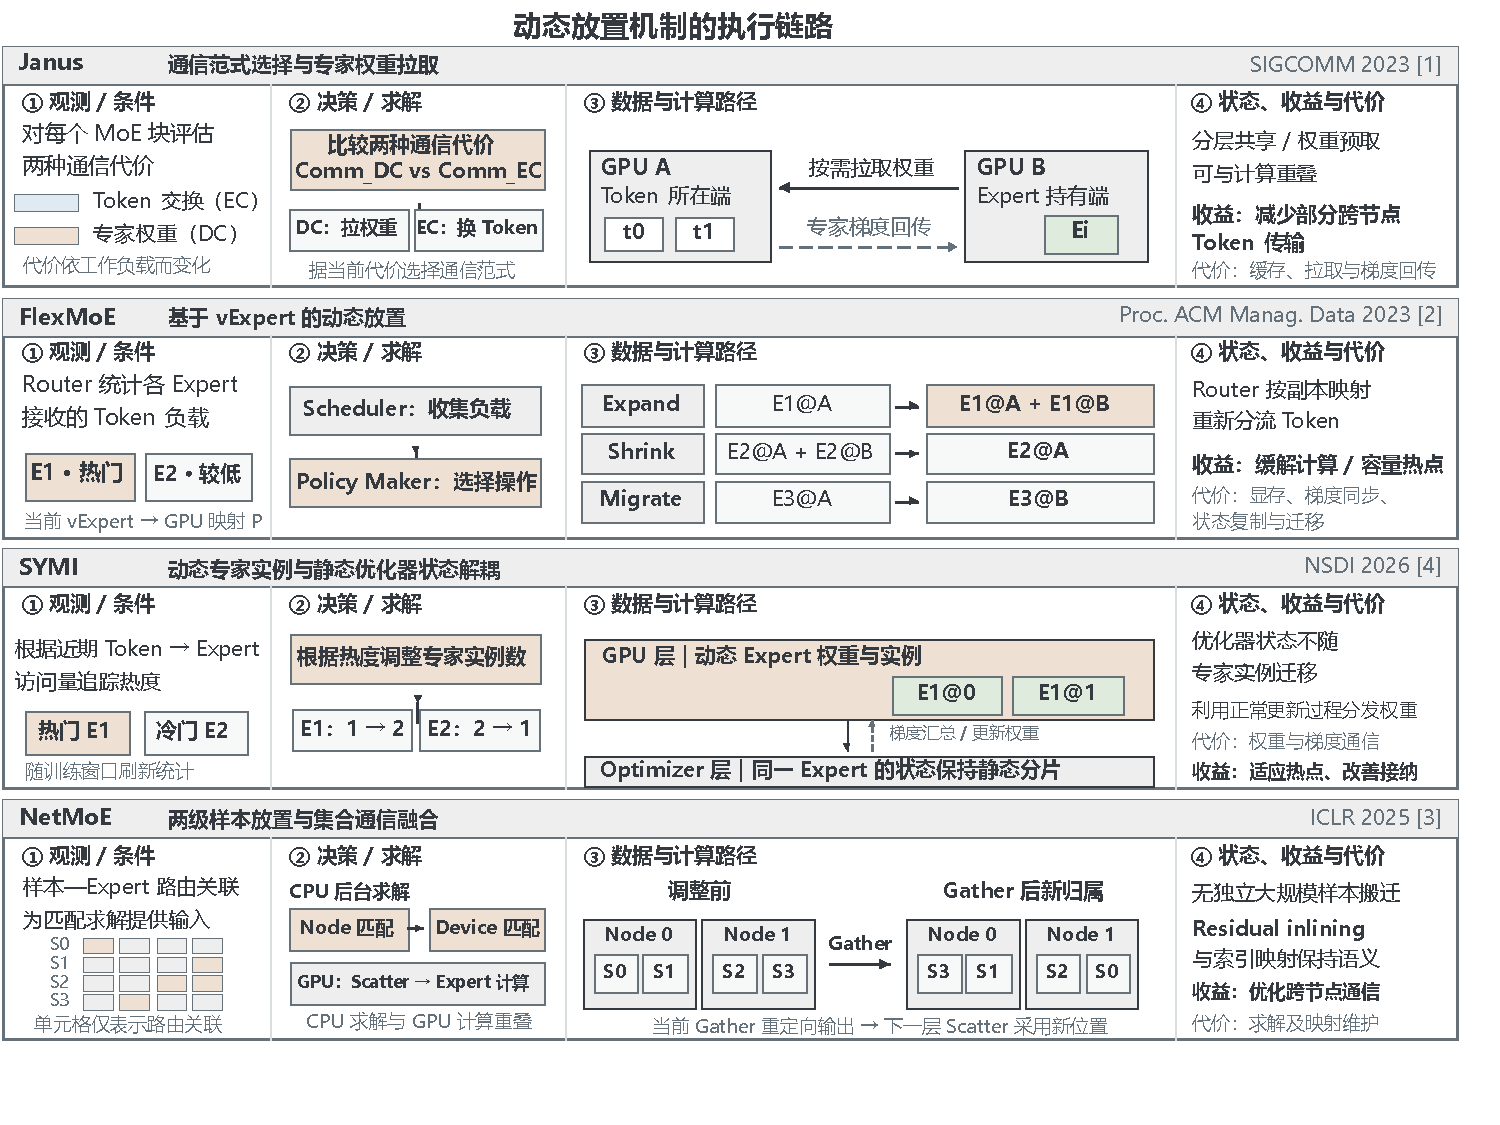
\includegraphics[width=\linewidth,trim=0 36pt 0 0,clip]{figures/figure2.pdf}
\caption{Janus、FlexMoE、SYMI 与 NetMoE 的主要执行链路。Janus 中 EC 表示 expert-centric，DC 表示 data-centric；四条泳道按代表工作组织，不作性能排名。根据文献 \cite{ref1,ref2,ref3,ref4} 整理绘制。}
\label{fig:mechanisms}
\end{figure}

\begin{table}[!t]
\centering
\caption{动态放置机制的条件化比较}
\label{tab:mechanism-comparison}
\footnotesize
\setlength{\tabcolsep}{2pt}
\renewcommand{\arraystretch}{1.12}
\begin{tabularx}{\linewidth}{>{\raggedright\arraybackslash}p{0.12\linewidth} >{\raggedright\arraybackslash}p{0.11\linewidth} >{\raggedright\arraybackslash}p{0.14\linewidth} >{\raggedright\arraybackslash}p{0.12\linewidth} >{\raggedright\arraybackslash}p{0.16\linewidth} >{\raggedright\arraybackslash}p{0.18\linewidth} >{\raggedright\arraybackslash}X}
\toprule
研究类别 & 代表工作 & 改变对象 & 主要瓶颈 & 关键收益来源 & 新增成本 & 典型适用条件 \\
\midrule
数据中心化专家拉取 & Janus\cite{ref1} & 专家权重与缓存位置 & token 跨节点搬运 & 用权重拉取替代部分 token 交换 & 权重搬运、缓存、拷贝、反向梯度回传 & 权重相对 token 数据较小且可复用 \\
动态专家复制/迁移 & FasterMoE\cite{ref5}、FlexMoE\cite{ref2}、SYMI\cite{ref4} & 热门专家副本和状态布局 & 专家计算或容量热点 & 增加热门专家的计算槽位 & 显存、权重更新、梯度同步、状态管理 & 热点持续、同步预算和显存充足 \\
动态样本放置 & NetMoE\cite{ref3} & 样本的节点或设备归属 & 跨节点网络路径 & 提高 token 与 expert 的局部性 & Gather 重定向、下一层 Scatter 联动、求解和映射维护 & 局部性明显、机内外带宽差异大 \\
通信调度与并行优化 & SmartMoE\cite{ref6}、Tutel\cite{ref7}、Lina\cite{ref8}、Parm\cite{ref9} & schedule、pipeline、micro-op & 已存在的通信暴露等待 & 调整并行策略、通信调度与竞争/重叠 & 切分、候选搜索和控制开销 & 放置不宜频繁改变或需作为共同执行层 \\
\bottomrule
\end{tabularx}
\end{table}

上述比较表明，两类局部性与专家负载偏斜并不等同。若路由局部性高且专家负载均衡，主要等待来自 token 的跨节点路径，样本重排更直接；复制专家会增加同步，却未必减少主要等待。若路由局部性低但某一专家在多个窗口持续过热，样本重排难以把随机访问变成本地访问，专家复制更可能缓解计算排队，但不能自动消除 token 传输。因此两类局部性与计算热点应分开诊断。

三类动作的净收益取决于调整能否隐藏：样本重排承担 Gather/Scatter 重定向与映射成本，专家复制需要权重、梯度和显存预算，expert fetch 需要缓存、权重复用与反向回传。只有节省的关键路径时间超过无法隐藏的求解、搬运、同步和切换成本，且局部性或热点足够持续，动态动作才值得执行。固定 routing、token 接纳规则和通信设置不变时，应比较 step-time 净收益；若改变容量与 token dropping，还要比较相同目标质量下的 time-to-convergence。SmartMoE、Tutel、Lina 和 Parm 表明调度可作共同执行层；路由快速变化时，保持布局并优化通信顺序可能更合适。

